\newpage
\section{TGGs in action}
\genHeader
\label{sect:TGGs_in_Action}

In order to run our TGG, it first needs to have something tangible to work with. We need to create an instance model\footnote{Refer to Part II, Section 3 for
review} of either one of our language metamodels, which can then be transformed into an instance model of the \emph{other} language (i.e., peform a forward or
backwards transformation). Since dictionaries are a much simpler structure, let's start with the backwards transformation, \texttt{dictionary} to
\texttt{LearningBox}.

\begin{itemize}

\item[$\blacktriangleright$] Navigate to \texttt{Dictionary\-Language/model/} and open \texttt{DictionaryLanguage.ecore}. Create a new
dynamic instance of a \texttt{Dictionary} named \texttt{target.xmi}. Don't quickly press \texttt{enter}! Make sure you save it under
\texttt{Learn\-ing\-Box\-To\-Dictionary\-In\-te\-gra\-tion/in\-stan\-ces/} (Fig.~\ref{fig:create_instance_dict}).

\begin{figure}[htbp]
\begin{center}
  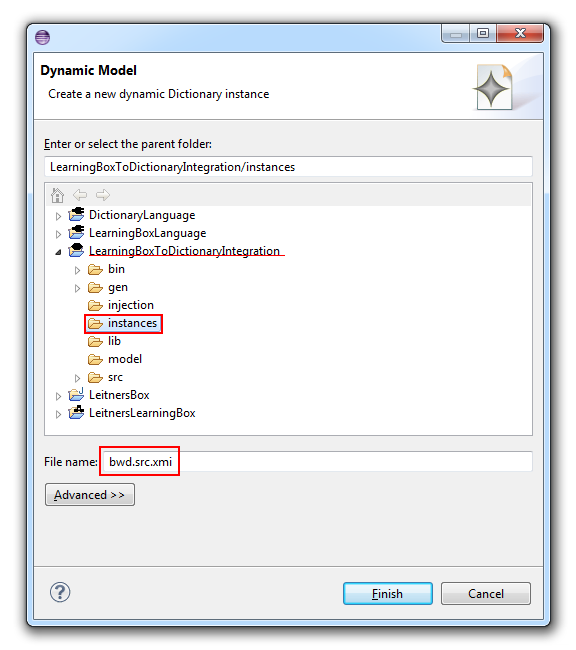
\includegraphics[width=0.8\textwidth]{eclipse_dictionaryInstance}
  \caption{Create a dynamic instance of \texttt{Dictionary}}
  \label{fig:create_instance_dict}
\end{center}
\end{figure}

\item[$\blacktriangleright$] Open \texttt{target.xmi}, and edit the \texttt{Dictionary} properties by setting \texttt{Title} to \texttt{English Numbers}.

\item[$\blacktriangleright$] Create two child \texttt{Entry} objects. Set \texttt{Content} of the first to \texttt{one : eins} and its
\texttt{Level} as \texttt{beginner}. Set the second with \texttt{eleven : elf} and \texttt{advanced} (Fig.~\ref{fig:dictionaryxmi}).

\begin{figure}[htbp]
\begin{center}
  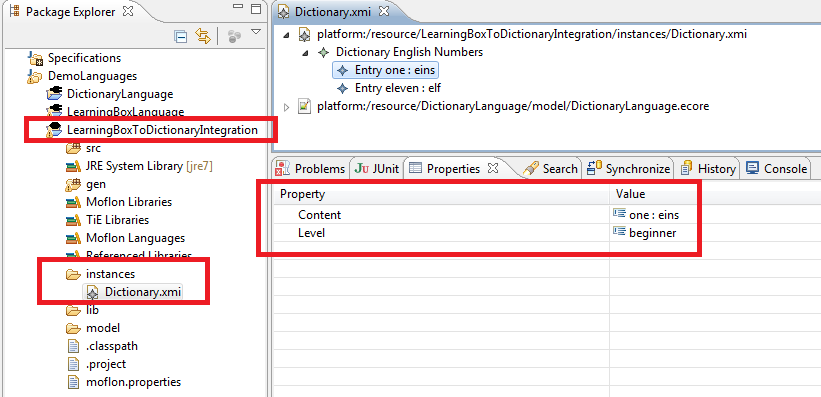
\includegraphics[width=\textwidth]{tgg26}
  \caption{Contents of the dictionary \update make smaller}
  \label{fig:dictionaryxmi}
\end{center}
\end{figure}

\item[$\blacktriangleright$] Run \texttt{TGGMain} as an application\footnote{Right-click, and navigate to ``Run as\ldots/Java Application''}, which can be found
in ``LearningBox\-To\-Dictionary\-In\-te\-gra\-tion\-/src''

\item[$\blacktriangleright$] In the eMoflon console below the editor, there should  one ``Unable to load instances/source.xmi'' error, followed by a success
message. Both of these makes sense -- our TGG first attempted a forward transformation but, given that it was missing the source instance, it was only able
to perform a transformation in one direction. Funnily enough however, we actually just created said source file. Since we have our LIST; LIST; and LIST, we
actually created the source graph. If you remember, this was one of our goals of TGG! Given one language, we wanted to be able to derive the other.  This
`error' then becomes an extremely easy fix, where we only need to find the generated instance and rename it.

\item[$\blacktriangleright$] Refresh the integration's \texttt{instances} folder. There should now be four new \texttt{xmi} files. You created \texttt{target},
\texttt{corr_BWD} is the correspondence graph between target and source, \texttt{protocol_BWD} is a listing of the attempted and successful steps taken in the
transformation, and \texttt{target.xmi_BWD} was the resulting graph. Open this file in the editor.

\item[$\blacktriangleright$] Expanding the platform, you can see a \texttt{Box} has been created, and it's \texttt{name} is the same as the \texttt{title} of
\texttt{Dictionary}, the result of the constraint set in our first rule, \texttt{BoxToDictionary}. The box also has three partition, despite
\texttt{Dictionary} not having any entries. This is because ..\update WORK ON THIS: may not actually be generating correctly..


As you can see, our \texttt{Dictionary} has been translated backward to a \texttt{Box} with the same name (\texttt{English Numbers}) and containing three
\texttt{Par\-ti\-tions} (as specified in \texttt{Box\-To\-Dictionary\-Rule}). The two \texttt{Entry} objects have been translated to \texttt{Card} objects as
specified in \texttt{CartToEntryRule}. The \texttt{face} and the \texttt{back} of the \texttt{Card}s are consistent with the \texttt{content}
of the corresponding \texttt{Entry}, e.g. \texttt{card.face = ``Question : one''} and \texttt{card.back = ``Answer : eins''}. The indices of the partitions
containing the cards are also consistent with the level of the entry, i.e., \texttt{0} for \texttt{beginner}, and \texttt{1} for \texttt{advanced}.

mention the graph viewer here!

\vspace{0.5cm}

Congratulations! You have successfully performed your first \emph{backward} transformation from your target model (dictionary) to your source (Learning box)
using TGGs! To show that the transformation is actually bidirectional however, lets edit the source model (thus resolving the error from above) and transform it
\emph{forward} to a new target model:


\item[$\blacktriangleright$] Make a copy of \texttt{target.xmi\_BWD.xmi} (the result of the backward transformation)
and rename it to \texttt{source.xmi}.
  
\item[$\blacktriangleright$] Open \texttt{source.xmi} and create some new \texttt{Card} objects in the \texttt{Partition}s (e.g., create a new \texttt{Card}
with \texttt{Card.face = ``Question : two''}, \texttt{Card.back = ``Answer : zwei''} in \texttt{Partition 0}).

\item[$\blacktriangleright$] Run the \texttt{TGGMain.java} again and inspect the result of the forward transformation, target model
\texttt{source.xmi\_FWD.xmi}.

\end{itemize}


To end this chapter on TGGs, lets check out another feature of eMolfon, the integrator visualizer! This will let us view the visualization of the created
triple model.

\newpage

\begin{itemize}

\item[$\blacktriangleright$] Right-click on \texttt{corr\_BWD.xmi} and choose ``eMoflon $\rightarrow$ Start Integrator'' which will open the window depicted in
Fig.~\ref{fig:integrator_start}.

\vspace{0.5cm}

\begin{figure}[htbp]
\begin{center}
  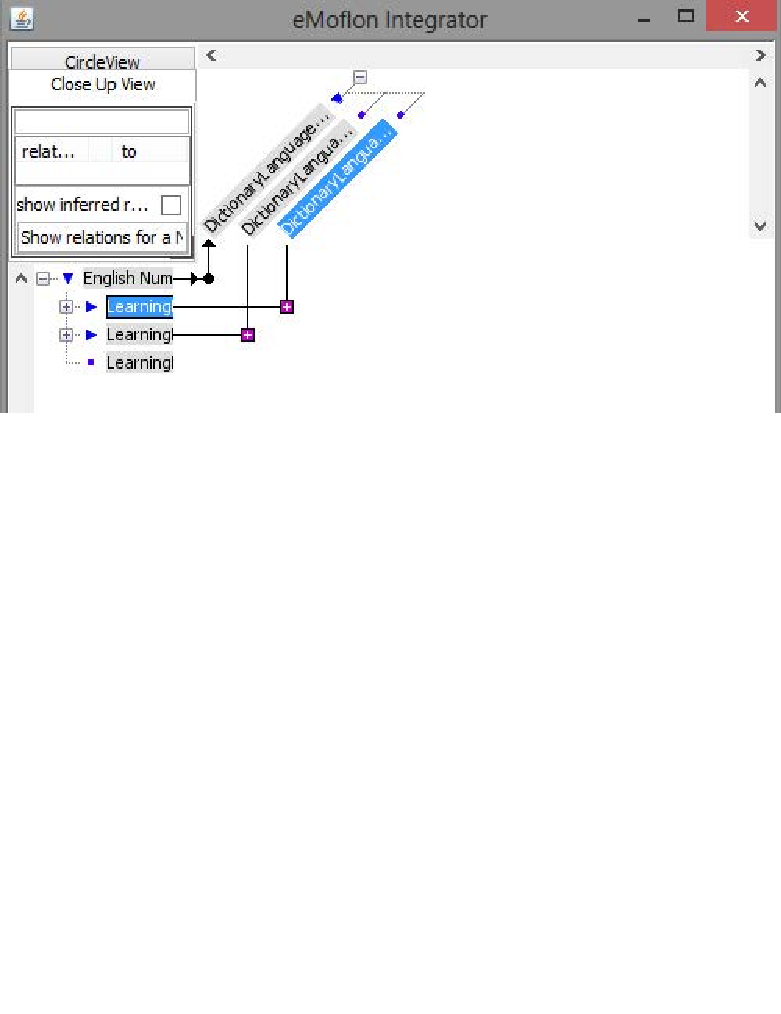
\includegraphics[width=0.7\textwidth]{integrator_start_view.pdf}
  \caption{Default view of the integrator}
  \label{fig:integrator_start}
\end{center}
\end{figure}

\item[$\blacktriangleright$] Drag and drop \texttt{protocol\_BWD.xmi} into the window. You will now see the controls explained in the lower part of the window 
(Fig.~\ref{fig:integrator_after_protocol}).

\begin{figure}[h!]
\begin{center}
  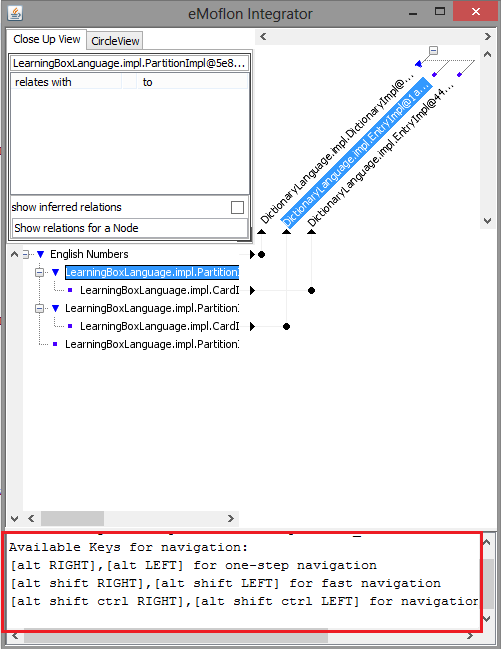
\includegraphics[width=0.6\textwidth]{integrator_after_protocol_insertion.png}
  \caption{Integrator after protocol insertion.}
  \label{fig:integrator_after_protocol}
\end{center}
\end{figure} 
\FloatBarrier

\item[$\blacktriangleright$] The integrator works as an ``offline'' debugger, working on the protocol (trace) of the transformation. You can use
\texttt{Alt+Right} to navigate forwards \emph{through} the transformation process, and \texttt{Alt+Left} to go backwards.  When you step through the
transformation, you will notice that some elements are highlighted with colours. These are the elements currently being processed. The colours have the
following definitions:
\begin{description}
  \item[Blue] The element is now about to be processed (is being ``looked at'').
  \vspace{0.5cm}
  \item[Yellow] The element cannot be transformed right now and has been queued for later transformation 
  (e.g., when transforming an Entry to a Card, the Box with partitions to put the 
  Card into must be translated first).
  \vspace{0.5cm}
  \item[Green] The object has just been created.
\end{description}

\end{itemize}
